% handouts/unit-circle/unit-circle.tex
% Algebra 2 / Trig unit circle handout. Two A4 pages, print double-sided:
%   page 1 -- the circle (radians, degrees, coordinates), coloured by family
%   page 2 -- sin / cos / tan table plus the tricks for remembering it
% Build: pdflatex unit-circle.tex (twice is not needed; no refs).
\documentclass[11pt]{article}
\usepackage[T1]{fontenc}
\usepackage[utf8]{inputenc}
\usepackage[default]{lato}
\usepackage[italic]{mathastext}
\usepackage[a4paper,top=1.4cm,bottom=1.3cm,left=1.5cm,right=1.5cm]{geometry}
\usepackage{amsmath,amssymb}
\usepackage[table]{xcolor}
\usepackage[most]{tcolorbox}
\usepackage{tikz}
\usepackage{array}
\usepackage{enumitem}
\pagestyle{empty}
\setlength{\parindent}{0pt}
\pgfdeclarelayer{fg}\pgfsetlayers{main,fg}

% Families: what the reference angle is. Same colours on both pages.
\definecolor{fsix}{HTML}{1A5FA8}   % pi/6  (30 deg)
\definecolor{ffour}{HTML}{4A8B23}  % pi/4  (45 deg)
\definecolor{fthree}{HTML}{C25E12} % pi/3  (60 deg)
\definecolor{faxis}{HTML}{3A3F44}  % quadrantal
\definecolor{ink}{HTML}{22272B}
\definecolor{soft}{HTML}{6B7680}

\newcommand{\hrt}[1]{\tfrac{\sqrt{#1}}{2}}

\newtcolorbox{tip}[2][]{enhanced, colback=#2!6, colframe=#2, boxrule=0pt,
  leftrule=3pt, arc=2pt, left=6pt, right=6pt, top=4pt, bottom=4pt,
  fonttitle=\bfseries\color{#2!85!black}, coltitle=#2!85!black,
  attach title to upper={\par\smallskip}, before skip=6pt, after skip=6pt, #1}

\begin{document}
\color{ink}

% =============================== PAGE 1 =====================================
{\Huge\bfseries The Unit Circle}\hfill{\large Name \rule{5cm}{0.4pt}}\par
\vspace{2pt}
{\large Radius $1$.\enspace Every point is $(\cos\theta,\ \sin\theta)$ \;=\; $(x,\ y)$.}\par
\vspace{4pt}

\begin{center}
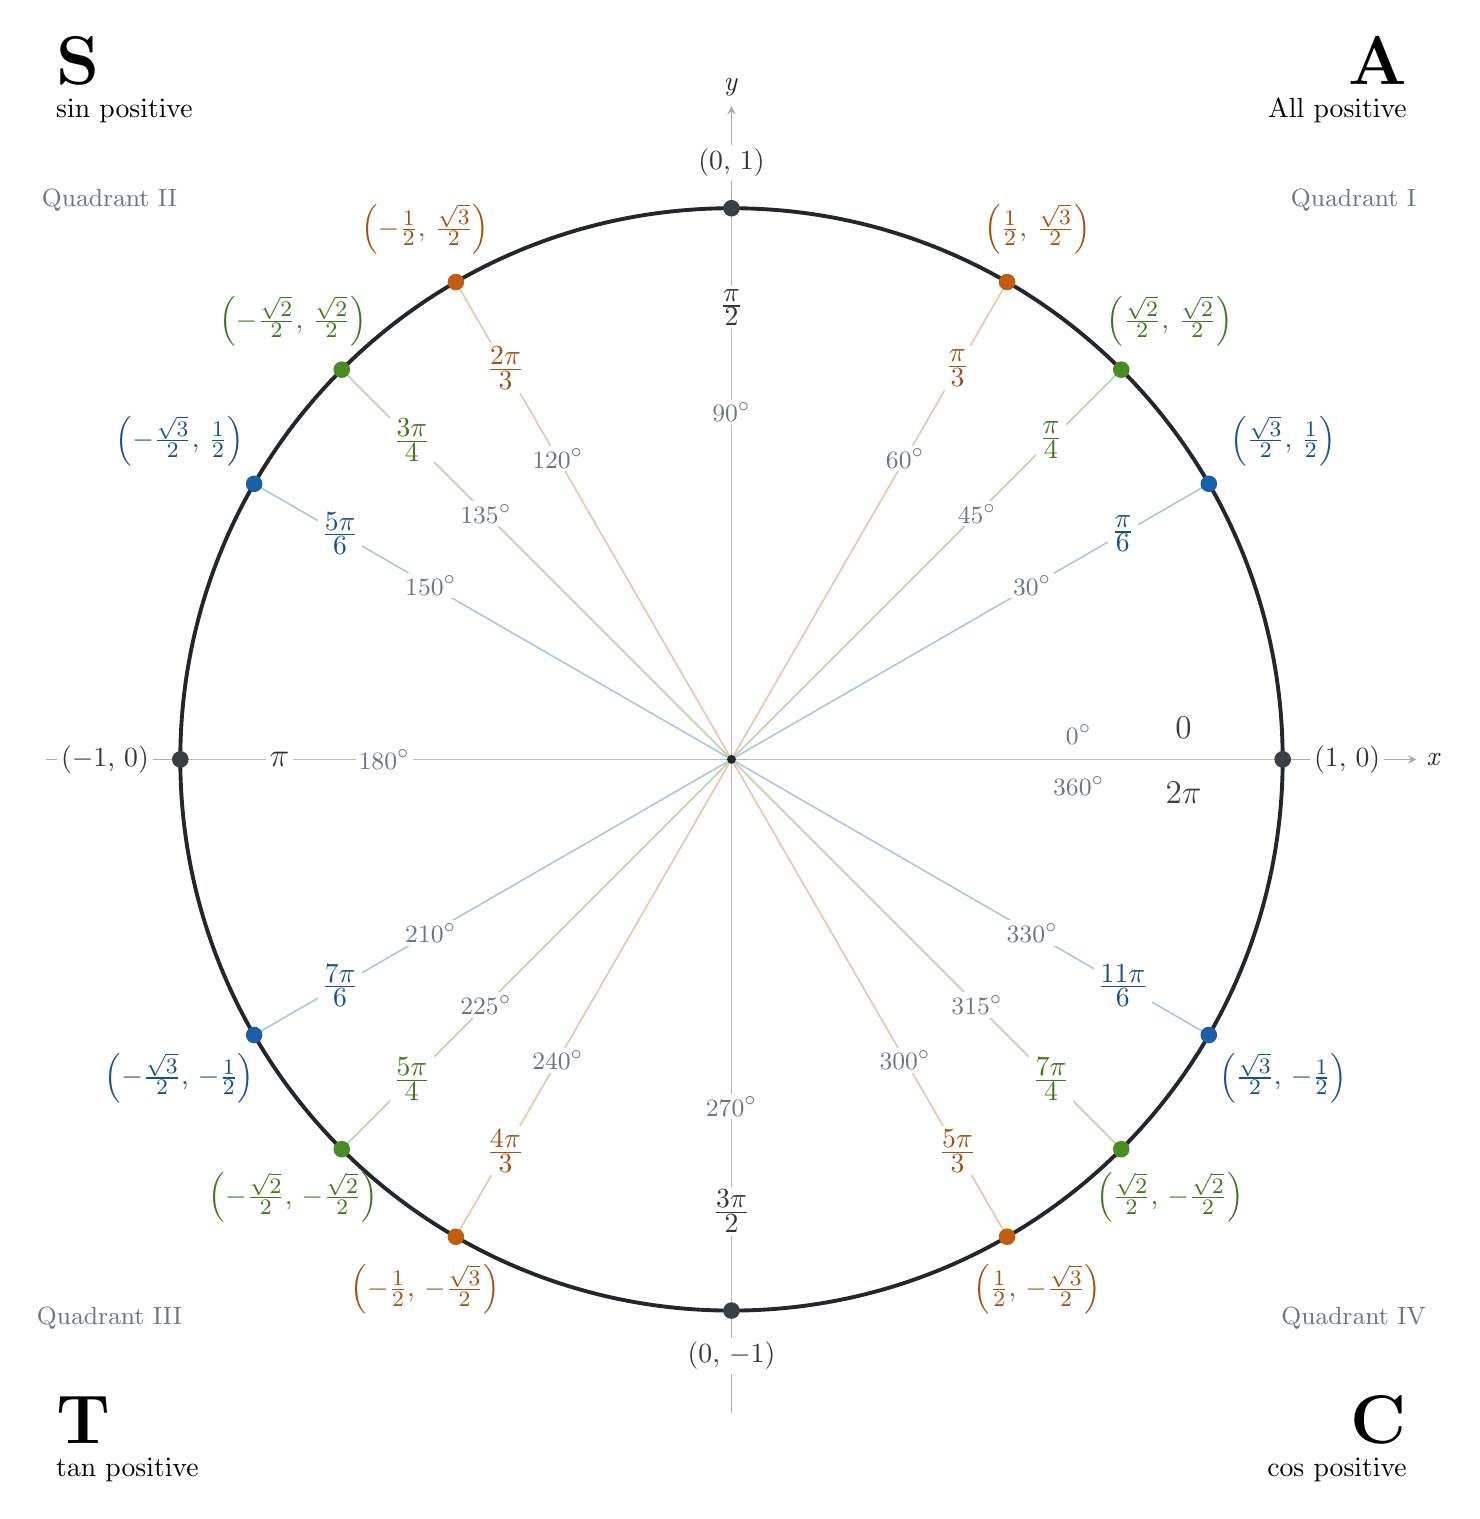
\begin{tikzpicture}[x=1cm,y=1cm]
  \def\R{7.0}

  % quadrant corners: signs (All Students Take Calculus)
  \begin{scope}[font=\large\bfseries]
    \node[anchor=north east, align=right] at (8.7,\R+2.3)
      {\Huge A\\[-2pt]\normalsize\mdseries All positive};
    \node[anchor=north west, align=left] at (-8.7,\R+2.3)
      {\Huge S\\[-2pt]\normalsize\mdseries $\sin$ positive};
    \node[anchor=south west, align=left] at (-8.7,-\R-2.3)
      {\Huge T\\[-2pt]\normalsize\mdseries $\tan$ positive};
    \node[anchor=south east, align=right] at (8.7,-\R-2.3)
      {\Huge C\\[-2pt]\normalsize\mdseries $\cos$ positive};
  \end{scope}
  \node[soft, font=\small] at (-7.9,\R+0.1) {Quadrant II};
  \node[soft, font=\small] at ( 7.9,\R+0.1) {Quadrant I};
  \node[soft, font=\small] at (-7.9,-\R-0.1) {Quadrant III};
  \node[soft, font=\small] at ( 7.9,-\R-0.1) {Quadrant IV};

  % axes, then the circle on the top layer so no label box can cut it
  \draw[soft!60, -stealth] (-\R-1.7,0) -- (\R+1.7,0) node[right, ink] {$x$};
  \draw[soft!60, -stealth] (0,-\R-1.3) -- (0,\R+1.3) node[above, ink] {$y$};
  \begin{pgfonlayer}{fg}
    \draw[ink, line width=1.4pt] (0,0) circle (\R);
  \end{pgfonlayer}

  % #1 degrees, #2 x, #3 y, #4 colour: ray, dot, coordinates
  \newcommand{\pt}[4]{%
    \pgfmathsetmacro{\anc}{#1+180}%
    \draw[#4!35, line width=0.6pt] (0,0) -- (#1:\R);
    \begin{pgfonlayer}{fg}\fill[#4] (#1:\R) circle (3pt);\end{pgfonlayer}
    \node[anchor=\anc, fill=white, inner sep=1.5pt, text=#4!85!black, font=\normalsize]
      at (#1:\R+0.34) {$\left(#2,\, #3\right)$};
  }
  % #1 degrees, #2 radians, #3 colour: labels inside the circle
  \newcommand{\lbl}[3]{%
    \node[fill=white, inner sep=1.2pt, text=#3!85!black, font=\large]
      at (#1:0.82*\R) {$#2$};
    \node[fill=white, inner sep=1pt, text=soft, font=\small]
      at (#1:0.63*\R) {$#1^\circ$};
  }
  \newcommand{\ang}[6]{\pt{#1}{#3}{#4}{#6}\lbl{#1}{#2}{#6}}

  \pt{0}{1}{0}{faxis}
  \ang{30}{\frac{\pi}{6}}{\hrt3}{\tfrac12}{}{fsix}
  \ang{45}{\frac{\pi}{4}}{\hrt2}{\hrt2}{}{ffour}
  \ang{60}{\frac{\pi}{3}}{\tfrac12}{\hrt3}{}{fthree}
  \ang{90}{\frac{\pi}{2}}{0}{1}{}{faxis}
  \ang{120}{\frac{2\pi}{3}}{-\tfrac12}{\hrt3}{}{fthree}
  \ang{135}{\frac{3\pi}{4}}{-\hrt2}{\hrt2}{}{ffour}
  \ang{150}{\frac{5\pi}{6}}{-\hrt3}{\tfrac12}{}{fsix}
  \ang{180}{\pi}{-1}{0}{}{faxis}
  \ang{210}{\frac{7\pi}{6}}{-\hrt3}{-\tfrac12}{}{fsix}
  \ang{225}{\frac{5\pi}{4}}{-\hrt2}{-\hrt2}{}{ffour}
  \ang{240}{\frac{4\pi}{3}}{-\tfrac12}{-\hrt3}{}{fthree}
  \ang{270}{\frac{3\pi}{2}}{0}{-1}{}{faxis}
  \ang{300}{\frac{5\pi}{3}}{\tfrac12}{-\hrt3}{}{fthree}
  \ang{315}{\frac{7\pi}{4}}{\hrt2}{-\hrt2}{}{ffour}
  \ang{330}{\frac{11\pi}{6}}{\hrt3}{-\tfrac12}{}{fsix}

  % 0 and 2pi share a point: 0 above the axis, 2pi below
  \node[text=faxis, font=\large] at (0.82*\R,0.4) {$0$};
  \node[text=soft, font=\small] at (0.63*\R,0.32) {$0^\circ$};
  \node[text=faxis, font=\large] at (0.82*\R,-0.42) {$2\pi$};
  \node[text=soft, font=\small] at (0.63*\R,-0.34) {$360^\circ$};

  \fill[ink] (0,0) circle (1.6pt);
\end{tikzpicture}
\end{center}

\vspace{-2pt}
\begin{center}
\renewcommand{\arraystretch}{1.3}
\begin{tabular}{@{}l@{\qquad}l@{\qquad}l@{\qquad}l@{}}
  \textcolor{fsix}{\large$\bullet$}\ \textbf{\textcolor{fsix}{denominator 6}}
  & \textcolor{ffour}{\large$\bullet$}\ \textbf{\textcolor{ffour}{denominator 4}}
  & \textcolor{fthree}{\large$\bullet$}\ \textbf{\textcolor{fthree}{denominator 3}}
  & \textcolor{faxis}{\large$\bullet$}\ \textbf{on an axis} \\
  \small reference angle $\frac{\pi}{6}=30^\circ$
  & \small reference angle $\frac{\pi}{4}=45^\circ$
  & \small reference angle $\frac{\pi}{3}=60^\circ$
  & \small values are $0,\ \pm1$ \\
  \small values $\tfrac12$ and $\hrt3$
  & \small values $\hrt2$ and $\hrt2$
  & \small values $\tfrac12$ and $\hrt3$
  & \\
\end{tabular}
\end{center}

\newpage
% =============================== PAGE 2 =====================================
{\Huge\bfseries Unit Circle Values}\par
\vspace{2pt}
{\large $\sin\theta = y$,\quad $\cos\theta = x$,\quad
$\tan\theta = \dfrac{\sin\theta}{\cos\theta} = \dfrac{y}{x}$ \;(the slope of the radius)}\par
\vspace{8pt}

\begin{minipage}[t]{0.535\textwidth}
\vspace{0pt}
\renewcommand{\arraystretch}{1.72}
\setlength{\tabcolsep}{7pt}
\newcommand{\rw}[6]{\rowcolor{#6!9}\textcolor{#6!85!black}{$#1^\circ$} &
  \textcolor{#6!85!black}{$#2$} & $#3$ & $#4$ & $#5$ \\}
\begin{tabular}{@{}>{\centering\arraybackslash}p{1.05cm}
  >{\centering\arraybackslash}p{1.15cm}
  >{\centering\arraybackslash}p{1.25cm}
  >{\centering\arraybackslash}p{1.25cm}
  >{\centering\arraybackslash}p{1.45cm}@{}}
  \rowcolor{ink}\textcolor{white}{\bfseries deg} & \textcolor{white}{\bfseries rad}
  & \textcolor{white}{$\boldsymbol{\sin\theta}$} & \textcolor{white}{$\boldsymbol{\cos\theta}$}
  & \textcolor{white}{$\boldsymbol{\tan\theta}$} \\
  \rw{0}{0}{0}{1}{0}{faxis}
  \rw{30}{\frac{\pi}{6}}{\tfrac12}{\hrt3}{\tfrac{\sqrt3}{3}}{fsix}
  \rw{45}{\frac{\pi}{4}}{\hrt2}{\hrt2}{1}{ffour}
  \rw{60}{\frac{\pi}{3}}{\hrt3}{\tfrac12}{\sqrt3}{fthree}
  \rw{90}{\frac{\pi}{2}}{1}{0}{\text{undefined}}{faxis}
  \rw{120}{\frac{2\pi}{3}}{\hrt3}{-\tfrac12}{-\sqrt3}{fthree}
  \rw{135}{\frac{3\pi}{4}}{\hrt2}{-\hrt2}{-1}{ffour}
  \rw{150}{\frac{5\pi}{6}}{\tfrac12}{-\hrt3}{-\tfrac{\sqrt3}{3}}{fsix}
  \rw{180}{\pi}{0}{-1}{0}{faxis}
  \rw{210}{\frac{7\pi}{6}}{-\tfrac12}{-\hrt3}{\tfrac{\sqrt3}{3}}{fsix}
  \rw{225}{\frac{5\pi}{4}}{-\hrt2}{-\hrt2}{1}{ffour}
  \rw{240}{\frac{4\pi}{3}}{-\hrt3}{-\tfrac12}{\sqrt3}{fthree}
  \rw{270}{\frac{3\pi}{2}}{-1}{0}{\text{undefined}}{faxis}
  \rw{300}{\frac{5\pi}{3}}{-\hrt3}{\tfrac12}{-\sqrt3}{fthree}
  \rw{315}{\frac{7\pi}{4}}{-\hrt2}{\hrt2}{-1}{ffour}
  \rw{330}{\frac{11\pi}{6}}{-\tfrac12}{\hrt3}{-\tfrac{\sqrt3}{3}}{fsix}
\end{tabular}
\end{minipage}\hfill
\begin{minipage}[t]{0.435\textwidth}
\vspace{0pt}
\begin{tip}[title={The square-root ladder}, before skip=0pt]{fsix}
Learn one line. Everything else is signs.\par\smallskip
\renewcommand{\arraystretch}{1.6}\setlength{\tabcolsep}{3.2pt}
\begin{tabular}{@{}r|ccccc@{}}
  $\theta$ & $0^\circ$ & $30^\circ$ & $45^\circ$ & $60^\circ$ & $90^\circ$ \\\hline
  $\sin$ & $\frac{\sqrt0}{2}$ & $\frac{\sqrt1}{2}$ & $\frac{\sqrt2}{2}$ & $\frac{\sqrt3}{2}$ & $\frac{\sqrt4}{2}$ \\
  $\cos$ & $\frac{\sqrt4}{2}$ & $\frac{\sqrt3}{2}$ & $\frac{\sqrt2}{2}$ & $\frac{\sqrt1}{2}$ & $\frac{\sqrt0}{2}$ \\
\end{tabular}\par\smallskip
\small $\sin$ counts up $0,1,2,3,4$. $\cos$ counts down.
\end{tip}

\begin{tip}[title={The hand trick}]{ffour}
\small Left hand, palm toward you, fingers spread.
Pinky $=0^\circ$, ring $=30^\circ$, middle $=45^\circ$, index $=60^\circ$, thumb $=90^\circ$.\par\smallskip
Fold down the finger for your angle.\par\smallskip
\quad$\sin\theta = \dfrac{\sqrt{p}}{2}$,\ \ $p$ = fingers on the pinky side\par\smallskip
\quad$\cos\theta = \dfrac{\sqrt{t}}{2}$,\ \ $t$ = fingers on the thumb side\par\smallskip
\emph{Example:} fold the ring finger ($30^\circ$). 1 finger on the pinky side, 3 on the thumb side:
$\sin30^\circ=\frac{\sqrt1}{2}=\frac12$, $\cos30^\circ=\frac{\sqrt3}{2}$.
\end{tip}

\begin{tip}[title={Big or small?}]{fthree}
\small Near the $x$-axis, $y$ is small.\par
\quad $30^\circ$:\ \ $\sin=\tfrac12$,\ \ $\cos=\hrt3$\par\smallskip
Near the $y$-axis, $y$ is big.\par
\quad $60^\circ$:\ \ $\sin=\hrt3$,\ \ $\cos=\tfrac12$\par\smallskip
Check: $\frac{\sqrt3}{2}\approx0.87$ and $\frac{\sqrt2}{2}\approx0.71$.
\end{tip}
\end{minipage}

\vspace{6pt}
\begin{tip}[title={Any angle in three steps}]{faxis}
\begin{minipage}[t]{0.56\linewidth}
\small
\textbf{1. Family.} Look at the denominator: 6, 4 or 3 gives reference angle
$\frac{\pi}{6}$, $\frac{\pi}{4}$ or $\frac{\pi}{3}$.\par
\textbf{2. Size.} Read the value off the ladder.\par
\textbf{3. Sign.} Find the quadrant. Use \textbf{A}ll \textbf{S}tudents
\textbf{T}ake \textbf{C}alculus.
\end{minipage}\hfill
\begin{minipage}[t]{0.41\linewidth}
\small\emph{Example:} $\sin\dfrac{7\pi}{6}$\par\smallskip
denominator 6 $\to$ size $\tfrac12$\par
$\frac{7\pi}{6}$ is just past $\pi$ $\to$ Quadrant III\par
$\sin$ is negative there $\to$ \fbox{$-\tfrac12$}
\end{minipage}
\end{tip}

\begin{minipage}[t]{0.49\textwidth}
\begin{tip}[title={Where the numbers come from}, equal height group=bot]{fsix}
\centering
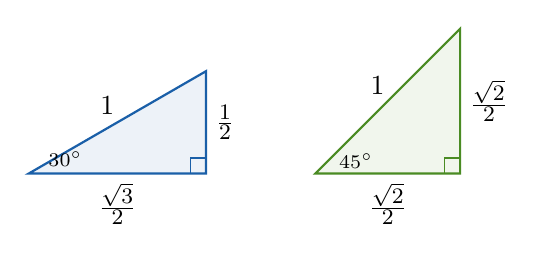
\begin{tikzpicture}[scale=2.6, font=\normalsize]
  \draw[fsix, thick, fill=fsix!8] (0,0) -- (0.866,0) -- (0.866,0.5) -- cycle;
  \draw[fsix] (0.79,0) -- (0.79,0.076) -- (0.866,0.076);
  \node[below] at (0.433,0) {$\hrt3$};
  \node[right] at (0.866,0.25) {$\tfrac12$};
  \node[above left, inner sep=1pt] at (0.433,0.27) {$1$};
  \node[right, inner sep=1pt] at (0.08,0.07) {\scriptsize$30^\circ$};
  \begin{scope}[xshift=1.4cm]
  \draw[ffour, thick, fill=ffour!8] (0,0) -- (0.707,0) -- (0.707,0.707) -- cycle;
  \draw[ffour] (0.631,0) -- (0.631,0.076) -- (0.707,0.076);
  \node[below] at (0.354,0) {$\hrt2$};
  \node[right] at (0.707,0.354) {$\hrt2$};
  \node[above left, inner sep=1pt] at (0.354,0.37) {$1$};
  \node[right, inner sep=1pt] at (0.1,0.06) {\scriptsize$45^\circ$};
  \end{scope}
\end{tikzpicture}\par\smallskip
\raggedright\small The radius is the hypotenuse, so it is $1$.
The legs are $\cos\theta$ and $\sin\theta$.
\end{tip}
\end{minipage}\hfill
\begin{minipage}[t]{0.49\textwidth}
\begin{tip}[title={Worth knowing}, equal height group=bot]{fthree}
\small
\renewcommand{\arraystretch}{1.55}
\begin{tabular}{@{}l@{\ \ }l@{}}
  Degrees $\to$ radians & $\times\ \pi/180^\circ$ \\
  Radians $\to$ degrees & $\times\ 180^\circ/\pi$ \\
  $1$ radian & $\approx 57.3^\circ$ \\
  Pythagoras & $\sin^2\theta+\cos^2\theta=1$ \\
  Same point & $\theta \pm 2\pi$ (coterminal) \\
  Negative angles & $\cos(-\theta)=\cos\theta$\\
   & $\sin(-\theta)=-\sin\theta$ \\
  Order & $(\cos,\sin)$: $c$ before $s$, $x$ before $y$
\end{tabular}
\end{tip}
\end{minipage}

\end{document}
